% !TeX spellcheck = it_IT
\documentclass[a4paper,12pt]{article}

\usepackage{alltt, fancyvrb, url}
\usepackage{graphicx}
\usepackage{algorithmic}
\usepackage[utf8]{inputenc}
\usepackage{titling}
\usepackage{fancyhdr}
\usepackage{fontenc}
\usepackage{amsmath,mathtools,algorithm}
\usepackage{amssymb}
\usepackage{longtable}
\usepackage{setspace}
\usepackage{listings}
\usepackage{color}
\usepackage{eurosym}
\usepackage{array}
\usepackage[referable]{threeparttablex}
\usepackage{pifont}

\newcommand{\cmark}{\ding{51}}
\newcommand{\xmark}{\ding{55}}

\usepackage[italian,hidelinks]{hyperref}

\usepackage[italian]{babel}
\usepackage[italian]{cleveref}


\pretitle{%
	\begin{center}
		\LARGE
	}
\posttitle{\end{center}}


\title{\Huge \textbf{Briscola Simulation} \\
	\vspace{10pt}
	\vspace{20pt}
}
\author{
	Gabriele Graffieti \\ \small \url{gabriele.graffieti@studio.unibo.it}
	\vspace{15pt}
	\\
	Alfredo Maffi \\ \small \url{alfredo.maffi@studio.unibo.it}
	\vspace{15pt}
	\\
	Manuel Peruzzi \\ \small \url{manuel.peruzzi@studio.unibo.it}
}

\date{}

\begin{document}

\maketitle
\pagenumbering{arabic}
\newpage
\tableofcontents
\newpage
\section{Idea}


\section{Analisi dei requisiti} \label{requirements-analysis}

In questo sezione verranno elencati ed analizzati i requisiti, funzionali e non, del sistema da realizzare. 

\subsection{Requisiti}

Lo scopo del progetto è quello di realizzare un sistema software in grado di simulare una partita di briscola a quattro giocatori. I giocatori dovranno sottostare al regolamento illustrato nella sezione  \emph{\hyperref[briscola-rules]{regole del gioco}} fornita in appendice. Ognuno di essi dovrà cooperare con il proprio compagno al meglio delle proprie capacità per poter vincere la partita. Più nel dettaglio, i requisiti funzionali sono i seguenti:
\begin{itemize}
	\item Le squadre devono essere scelte a caso, così come il primo giocatore ad inizio partita.
	\item Le carte del mazzo devono essere distribuite da una mazziere, seguendo l'ordine indicato nelle \emph{\hyperref[briscola-rules]{regole del gioco}} in appendice. Il mazziere, mano dopo mano, distribuirà carte fino ad esaurimento del mazzo.
	\item Un giocatore può iniziare a parlare con il compagno solamente quando è di mano ed è il primo della propria squadra a giocare per la mano corrente. Fa eccezione la prima mano, in cui non è consentito parlare.
	\item Quando un giocatore parla, tutti gli altri devono essere in grado di sentirlo. Inoltre, il compagno è sempre tenuto a rispondere.  Non sono ammessi \emph{bluff}: ogni giocatore, quando parla o risponde, è sempre obbligato a dire la verità.
	\item Ogni giocatore deve avere come obiettivo quello di massimizzare il punteggio della propria squadra, e non quello individuale.
	\item Ogni giocatore determina la propria giocata seguendo un propria logica interna, facendo affidamento su informazioni di varia natura. Tali informazioni sono costituite da:
	\begin{itemize}
		\item L'insieme delle carte che ha in mano.
		\item Eventuali carte giocate sul tavolo da gioco dagli altri giocatori in questa mano.
		\item Ciò che è stato detto dagli altri giocatori in questa mano.
		\item Le carte giocate nell'ultima presa, che saranno reperibili sul tavolo da gioco.
		\item Opzionalmente, le carte giocate nelle prese precedenti all'ultima.
		\item Opzionalmente, ciò che è stato detto dagli altri giocatori in precedenza.
	\end{itemize}
	\item Il tempo impiegato da un giocatore per decidere la prossima mossa non deve mai superare il tempo massimo di 2 secondi.
\end{itemize}

\subsection{Glossario} \label{glossary}

\begin{description}
	\item[Mazzo]: insieme di 40 carte disposte a pila in ordine casuale. Ogni carta è caratterizzata da un valore e un seme. I valori sono 10: comprendono i numeri da 1 a 7 e le figure fante, cavallo e re. I semi sono 4: denari, bastoni, spade e coppe.
	\item[Mazziere]: entità separata dai giocatori, avente l'unico scopo di distribuire le carte del mazzo ai giocatori stessi. 
	\item[Mano]: termine utilizzato per indicare un turno completo di gioco, in cui ogni giocatore gioca una carta a partire dal primo giocatore in senso antiorario. Il primo giocatore è colui che ha vinto l'ultima presa, ad eccezione del primo turno, dove viene scelto casualmente.
	\item[Presa]: l'insieme delle quattro carte sul tavolo al termine di una mano, che verranno assegnate al giocare che ha calato la carta dominante. Per carta dominante s'intende quella specificata nel regolamento in appendice.
	\item[Essere di mano]: un giocatore è di mano quando tocca a lui giocare una carta.
	\item[Fascia di valore]: raggruppamento di carte sulla base del loro valore. Le fasce sono tre: \emph{carico} (3 e asso), \emph{figura} (re, cavallo e fante) e \emph{liscia} (7, 6, 5, 4, 2).
	\item[Parlare]: scambio di informazioni tra due giocatori di una squadra. Il giocatore che \emph{parla} pone una domanda al compagno, il quale può rispondere in maniera binaria (``sì'' o ``no''). Tale domanda è finalizzata all'acquisizione di informazioni relative alle carte del compagno. Ogni domanda può contenere l'indicazione di una fascia di valore, di un seme o di entrambi: chi la riceve, risponde positivamente soltanto se possiede almeno una carta conforme all'indicazione. Seguono due esempi di domande lecite:
	\begin{itemize}
		\item "Hai una \emph{figura} di \emph{bastoni}?"
		\item "Hai una carta di \emph{denari}?"
	\end{itemize} 
	Presupponendo che chi riceve la domanda abbia in mano cavallo di bastoni, quattro di coppe e due di spade, risponderà positivamente alla prima domanda e negativamente alla seconda.   
	\item[Tavolo da gioco]: astrazione del tavolo fisico sul quale viene disputata la partita di briscola. Su di esso saranno posizionate le carte della mano corrente e la presa della mano precedente.
\end{description}

\subsection{Modello del dominio} \label{domain-model}

\subsubsection{Struttura}

Dai requisiti sopra elencati, è possibile individuare sei componenti all'interno del sistema:
\begin{itemize}
	\item Quattro giocatori, divisi in coppie in due squadre.
	\item Un mazziere, responsabile della distribuzione delle carte. \'E un'entità separata che non partecipa alla partita.
	\item Un tavolo da gioco, necessario per giocare carte e tenere memoria dell'ultima presa. 
\end{itemize}

Siccome i giocatori sono entità autonome con un proprio stato interno ed una capacità di \emph{reasoning} necessaria alla scelta delle carte da giocare, viene naturale modellarli come entità attive. Allo stesso modo, pur non avendo la stessa capacità di \emph{reasoning}, anche il mazziere è modellato come entità attiva. Infine, vien naturale modellare il tavolo come un'entità passiva, finalizzata a mantenere lo stato dell'ultima mano e di quella corrente. 

\subsubsection{Comportamento}

Di seguito è illustrato lo svolgimento di una partita, in modo da mettere in evidenza il comportamento del sistema e l'interazione tra i suoi componenti. Si presuppone che le due squadre siano già state formate e che i giocatori siano disposti come da regolamento.

\begin{enumerate}
	\item Il mazziere mischia il mazzo, distribuisce 3 carte ad ogni giocatore ed infine scopre una carta, il cui seme sarà la briscola per la partita corrente.
	\item Il primo giocatore, scelto casualmente, gioca una carta calandola sul tavolo, seguito dai restanti giocatori in senso antiorario.
	\item Quando tutte le quattro carte sono sul tavolo, queste vengono attribuite al giocatore vincente, che sarà il primo giocatore della prossima mano. A questo punto il mazziere distribuisce una carta ad ogni giocatore seguendo l'ordine della mano successiva, terminando così la mano corrente.
	\item Nelle seguenti mani, si procederà allo stesso modo (passi 2 e 3), con la possibilità di parlare da parte dei primi due giocatori di mano.
	\item Si procede fino all'esaurimento delle carte del mazzo e delle carte in mano ai giocatori. A questo punto, si procede al conteggio dei punti delle due squadre. Se una squadra ha totalizzato più di 60 punti è eletta vincitrice.
\end{enumerate}

Di seguito sono riportati due diagrammi a stati dai quali è possibile evincere comportamento dei giocatori e comportamento del mazziere rispettivamente in \autoref{player-state-diagram} e in \autoref{dealer-state-diagram}.

\begin{figure}[H]
	\centering
	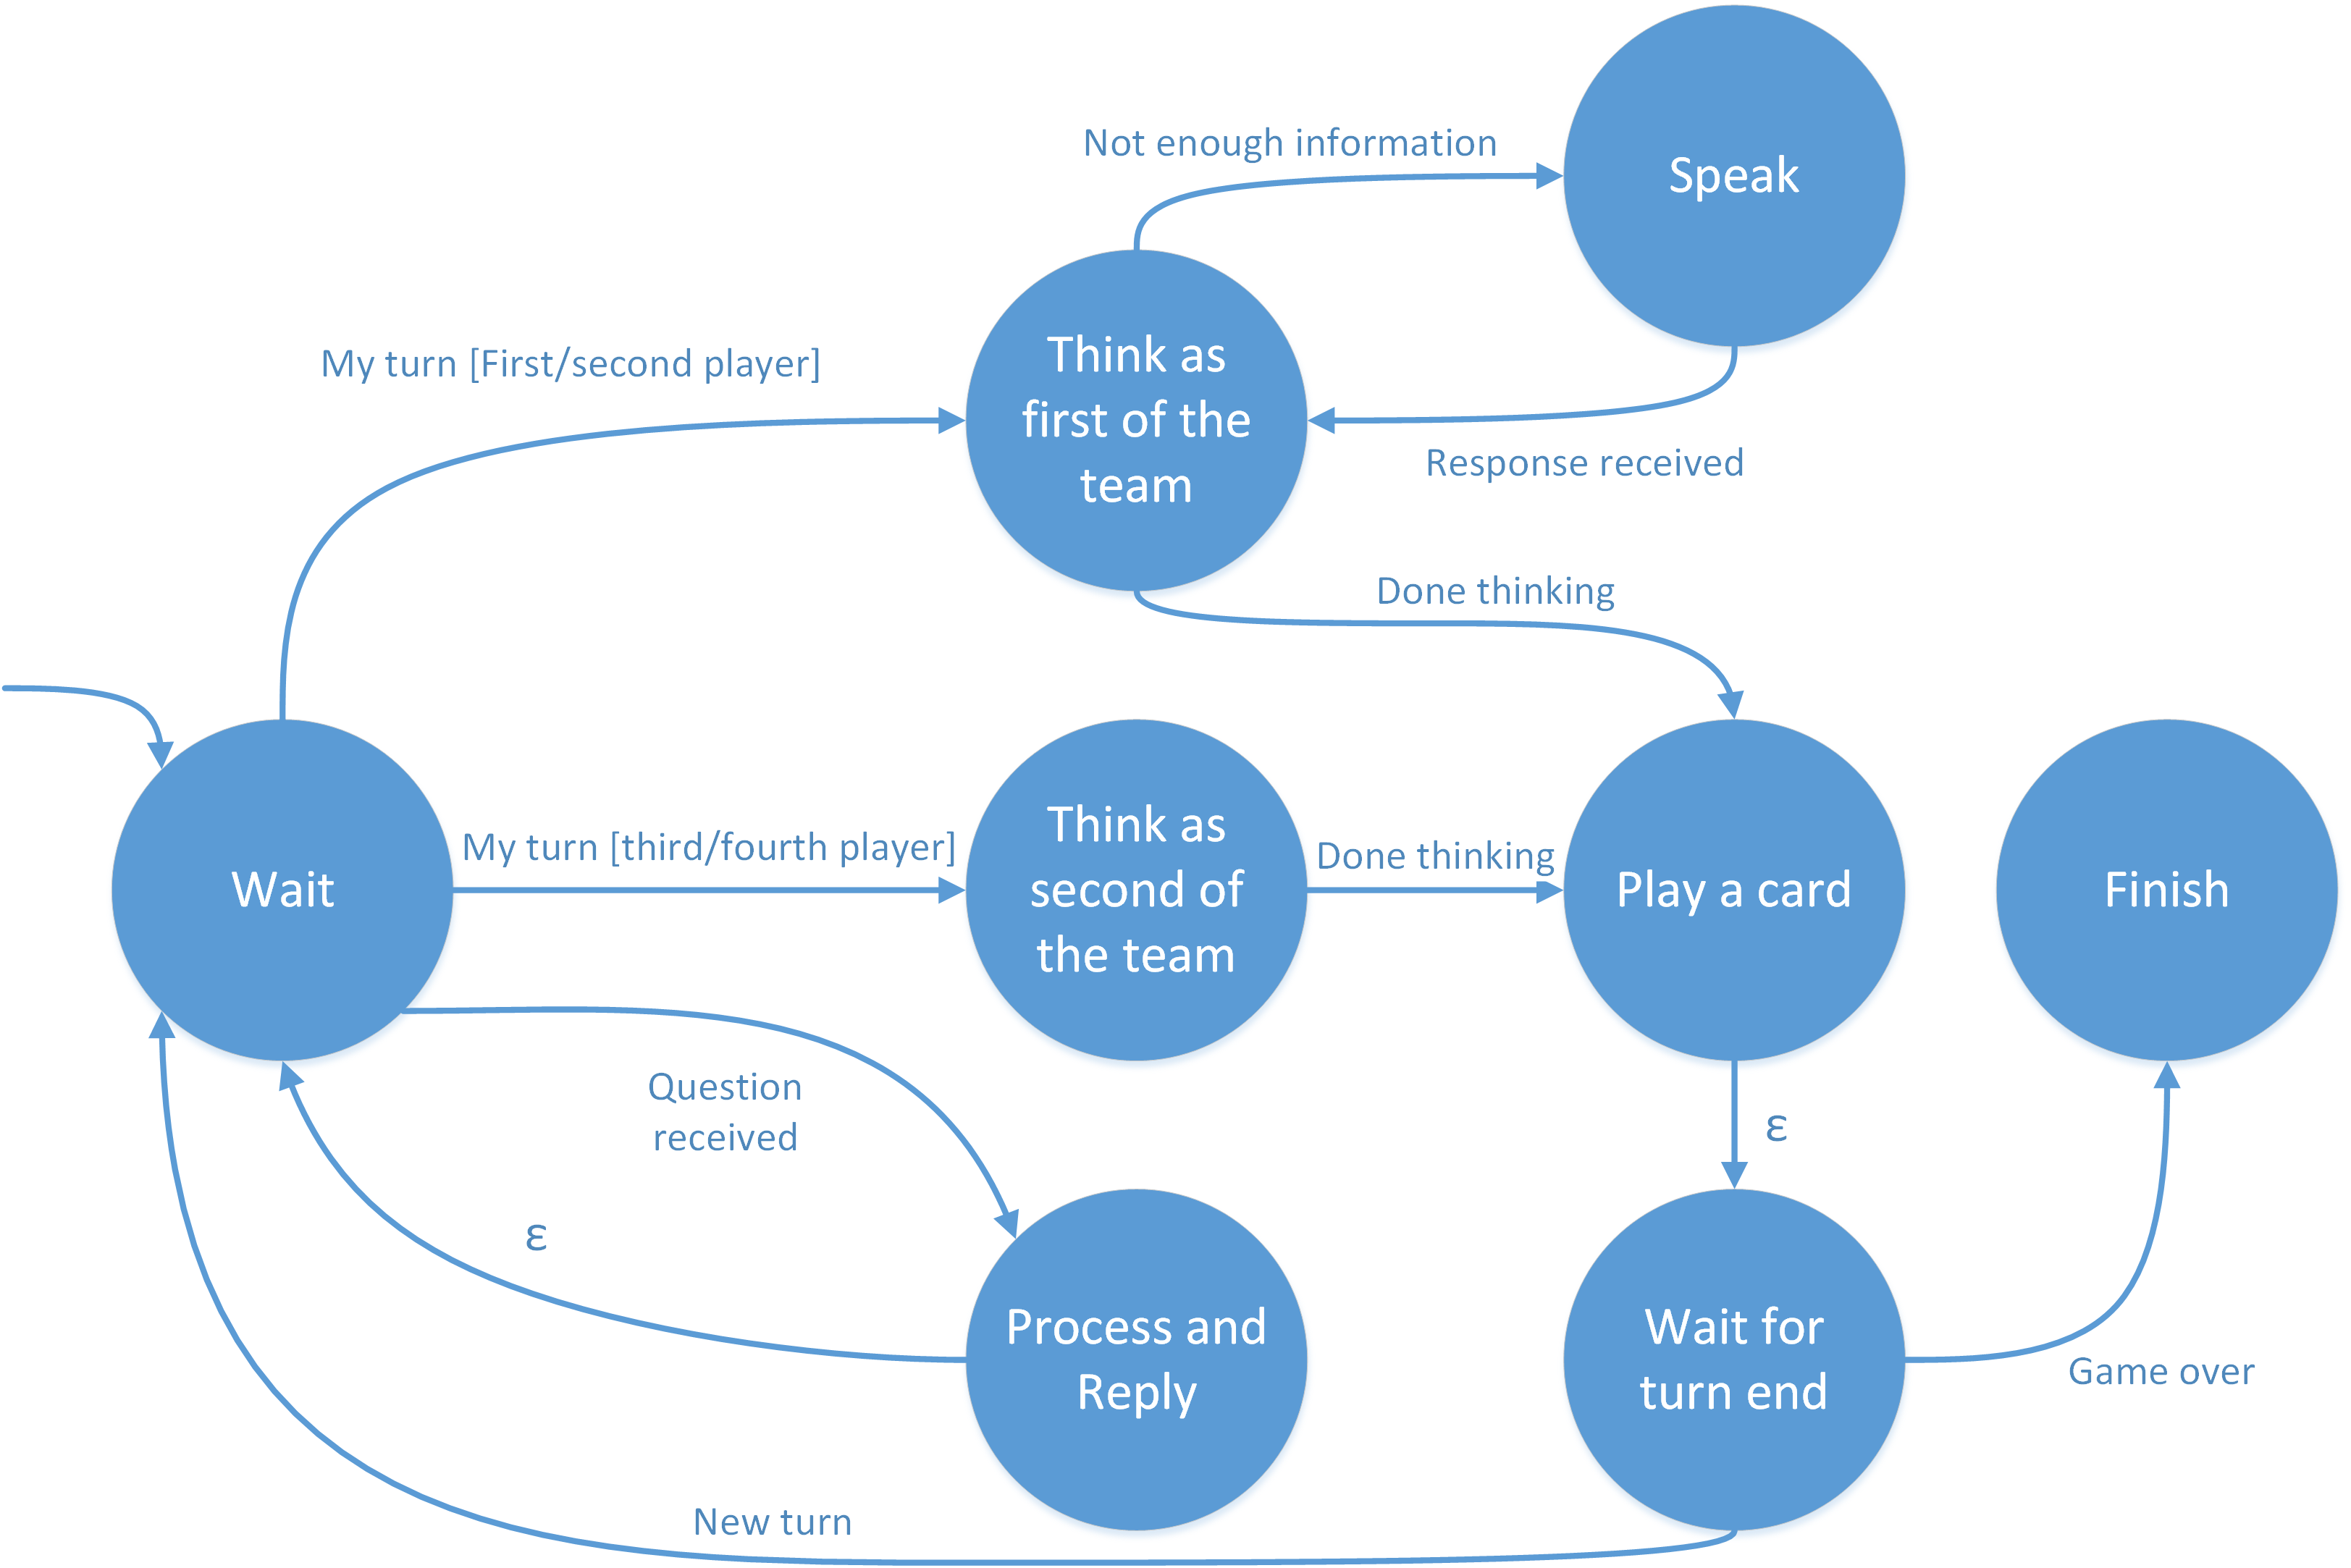
\includegraphics[width=140mm]{./img/player_state_diagram.png}
	\caption{Diagramma a stati di un giocatore.  \label{player-state-diagram}}
\end{figure}


\begin{figure}[H]
	\hspace*{-0.7in}
	\centering
	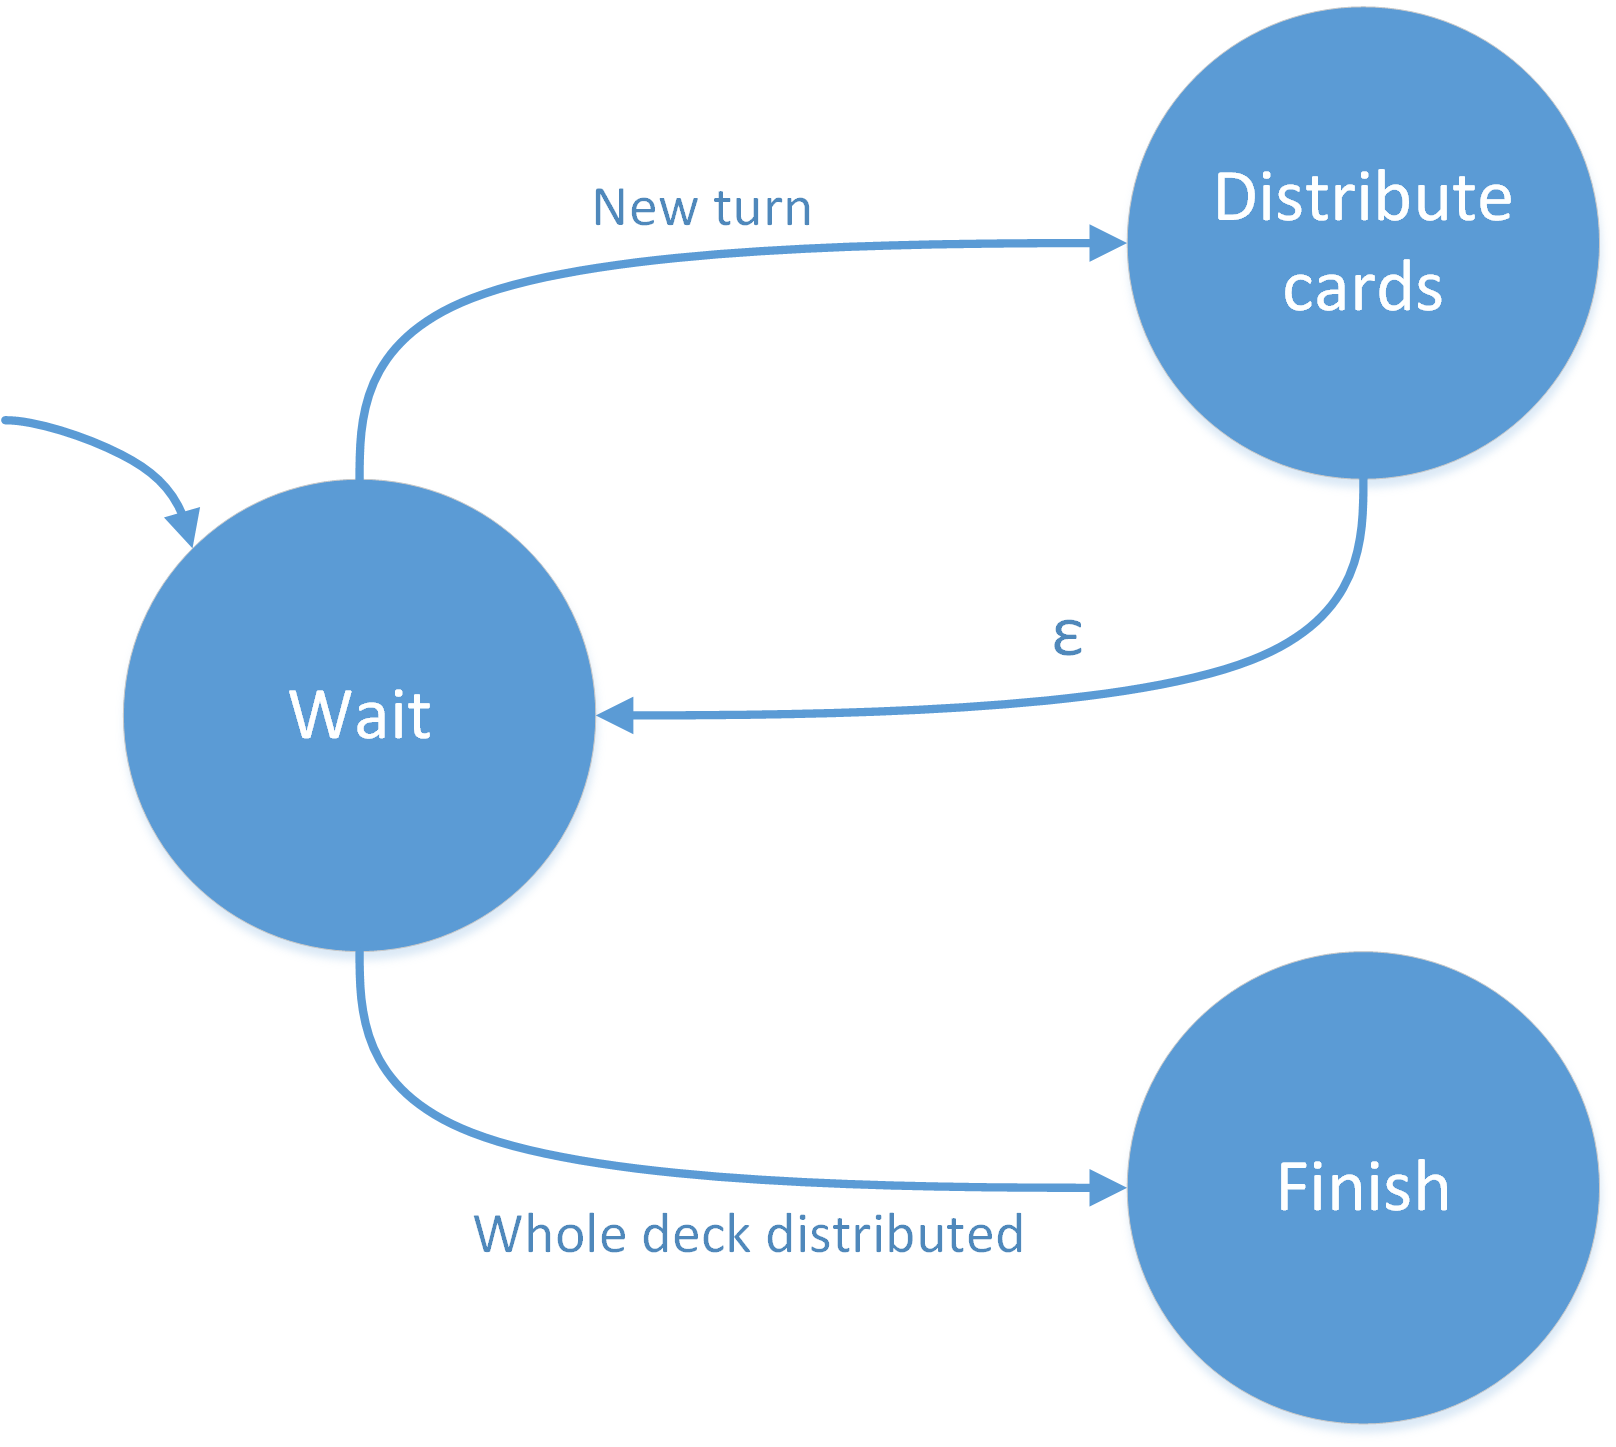
\includegraphics[width=70mm]{./img/dealer_state_diagram.png}
	\caption{Diagramma a stati del mazziere.  \label{dealer-state-diagram}}
\end{figure}

\subsubsection{Interazione}

Consultando i requisiti, è facile notare che l'interazione tra i componenti del sistema costituisce il punto focale del progetto, se non quello più delicato e complesso. Siccome dai requisiti stessi non è possibile evincere un schema di interazione, è necessaria un'analisi nel dettaglio per determinare lo schema migliore, effettuato nella prossima sezione.  

\section{Analisi del problema} \label{problem-analysis}
Il modello del dominio, individuato in \autoref{domain-model}, non risulta adeguatamente sviluppato per procedere alla fase di progettazione del sistema. I componenti individuati non sono sufficienti per un completo svolgimento di una partita. Un'importante funzionalità del sistema consiste nell'assegnamento di ogni presa al giocatore vincente, e nel conseguente conteggio finale dei punti accumulati dalle due squadre. Tale funzionalità non è ricoperta da nessuno dei componenti individuati. L'unico di essi che concettualmente potrebbe svolgere un tale compito è il tavolo da gioco. Le funzionalità espresse in precedenza implicano che il componente che ne è responsabile sia un'entità attiva con un proprio flusso di controllo. Il tavolo, modellato in precedenza come entità passiva, non risulta adeguato a svolgere tali mansioni. Perciò si rende necessaria l'introduzione di un nuovo componente, ovvero \emph{arbitro}.

Inoltre, dai requisiti non è chiaro in che modo le entità del sistema possano coordinarsi tra loro durante lo svolgimento di una partita. In particolare, non è specificata la modalità tramite la quale un giocatore sappia qual è il momento adatto per effettuare la sua giocata in una determinata mano. Allo stesso modo, non è indicato come il mazziere venga a conoscenza del momento in cui si conclude la fase di assegnazione della mano, per poi procedere alla distribuzione delle carte. Questa problematica potrebbe essere risolta in diversi modi:
\begin{itemize}
	\item \textbf{Introduzione di un orchestratore}: la coordinazione tra le entità del sistema potrebbe essere garantita dall'introduzione di un nuovo componente adibito.
	\item \textbf{Assegnamento del compito di orchestratore all'arbitro}: data la concezione di arbitro, non è difficile immaginare che possa essere proprio tale componente a fornire anche funzionalità di coordinazione di una partita.
	\item \textbf{Coordinazione tramite le informazioni sul tavolo}: siccome il tavolo è l'entità sulla quale si svolge la partita, esso potrebbe essere considerato come una sorgente di informazioni ed eventi, utilizzabili da giocatori, mazziere e arbitro per coordinarsi.
\end{itemize}
Fra le opzioni elencate, è sembrato più appropriato mettere in atto la seconda, attribuendo all'arbitro il ruolo di orchestratore della partita.

Sulla base di quanto discusso, in \autoref{general-sequence-diagram} è illustrato un diagramma di sequenza, in modo da mettere in evidenza l'interazione tra i componenti del sistema.


\begin{figure}[H]
	\hspace*{-0.7in}
	\centering
	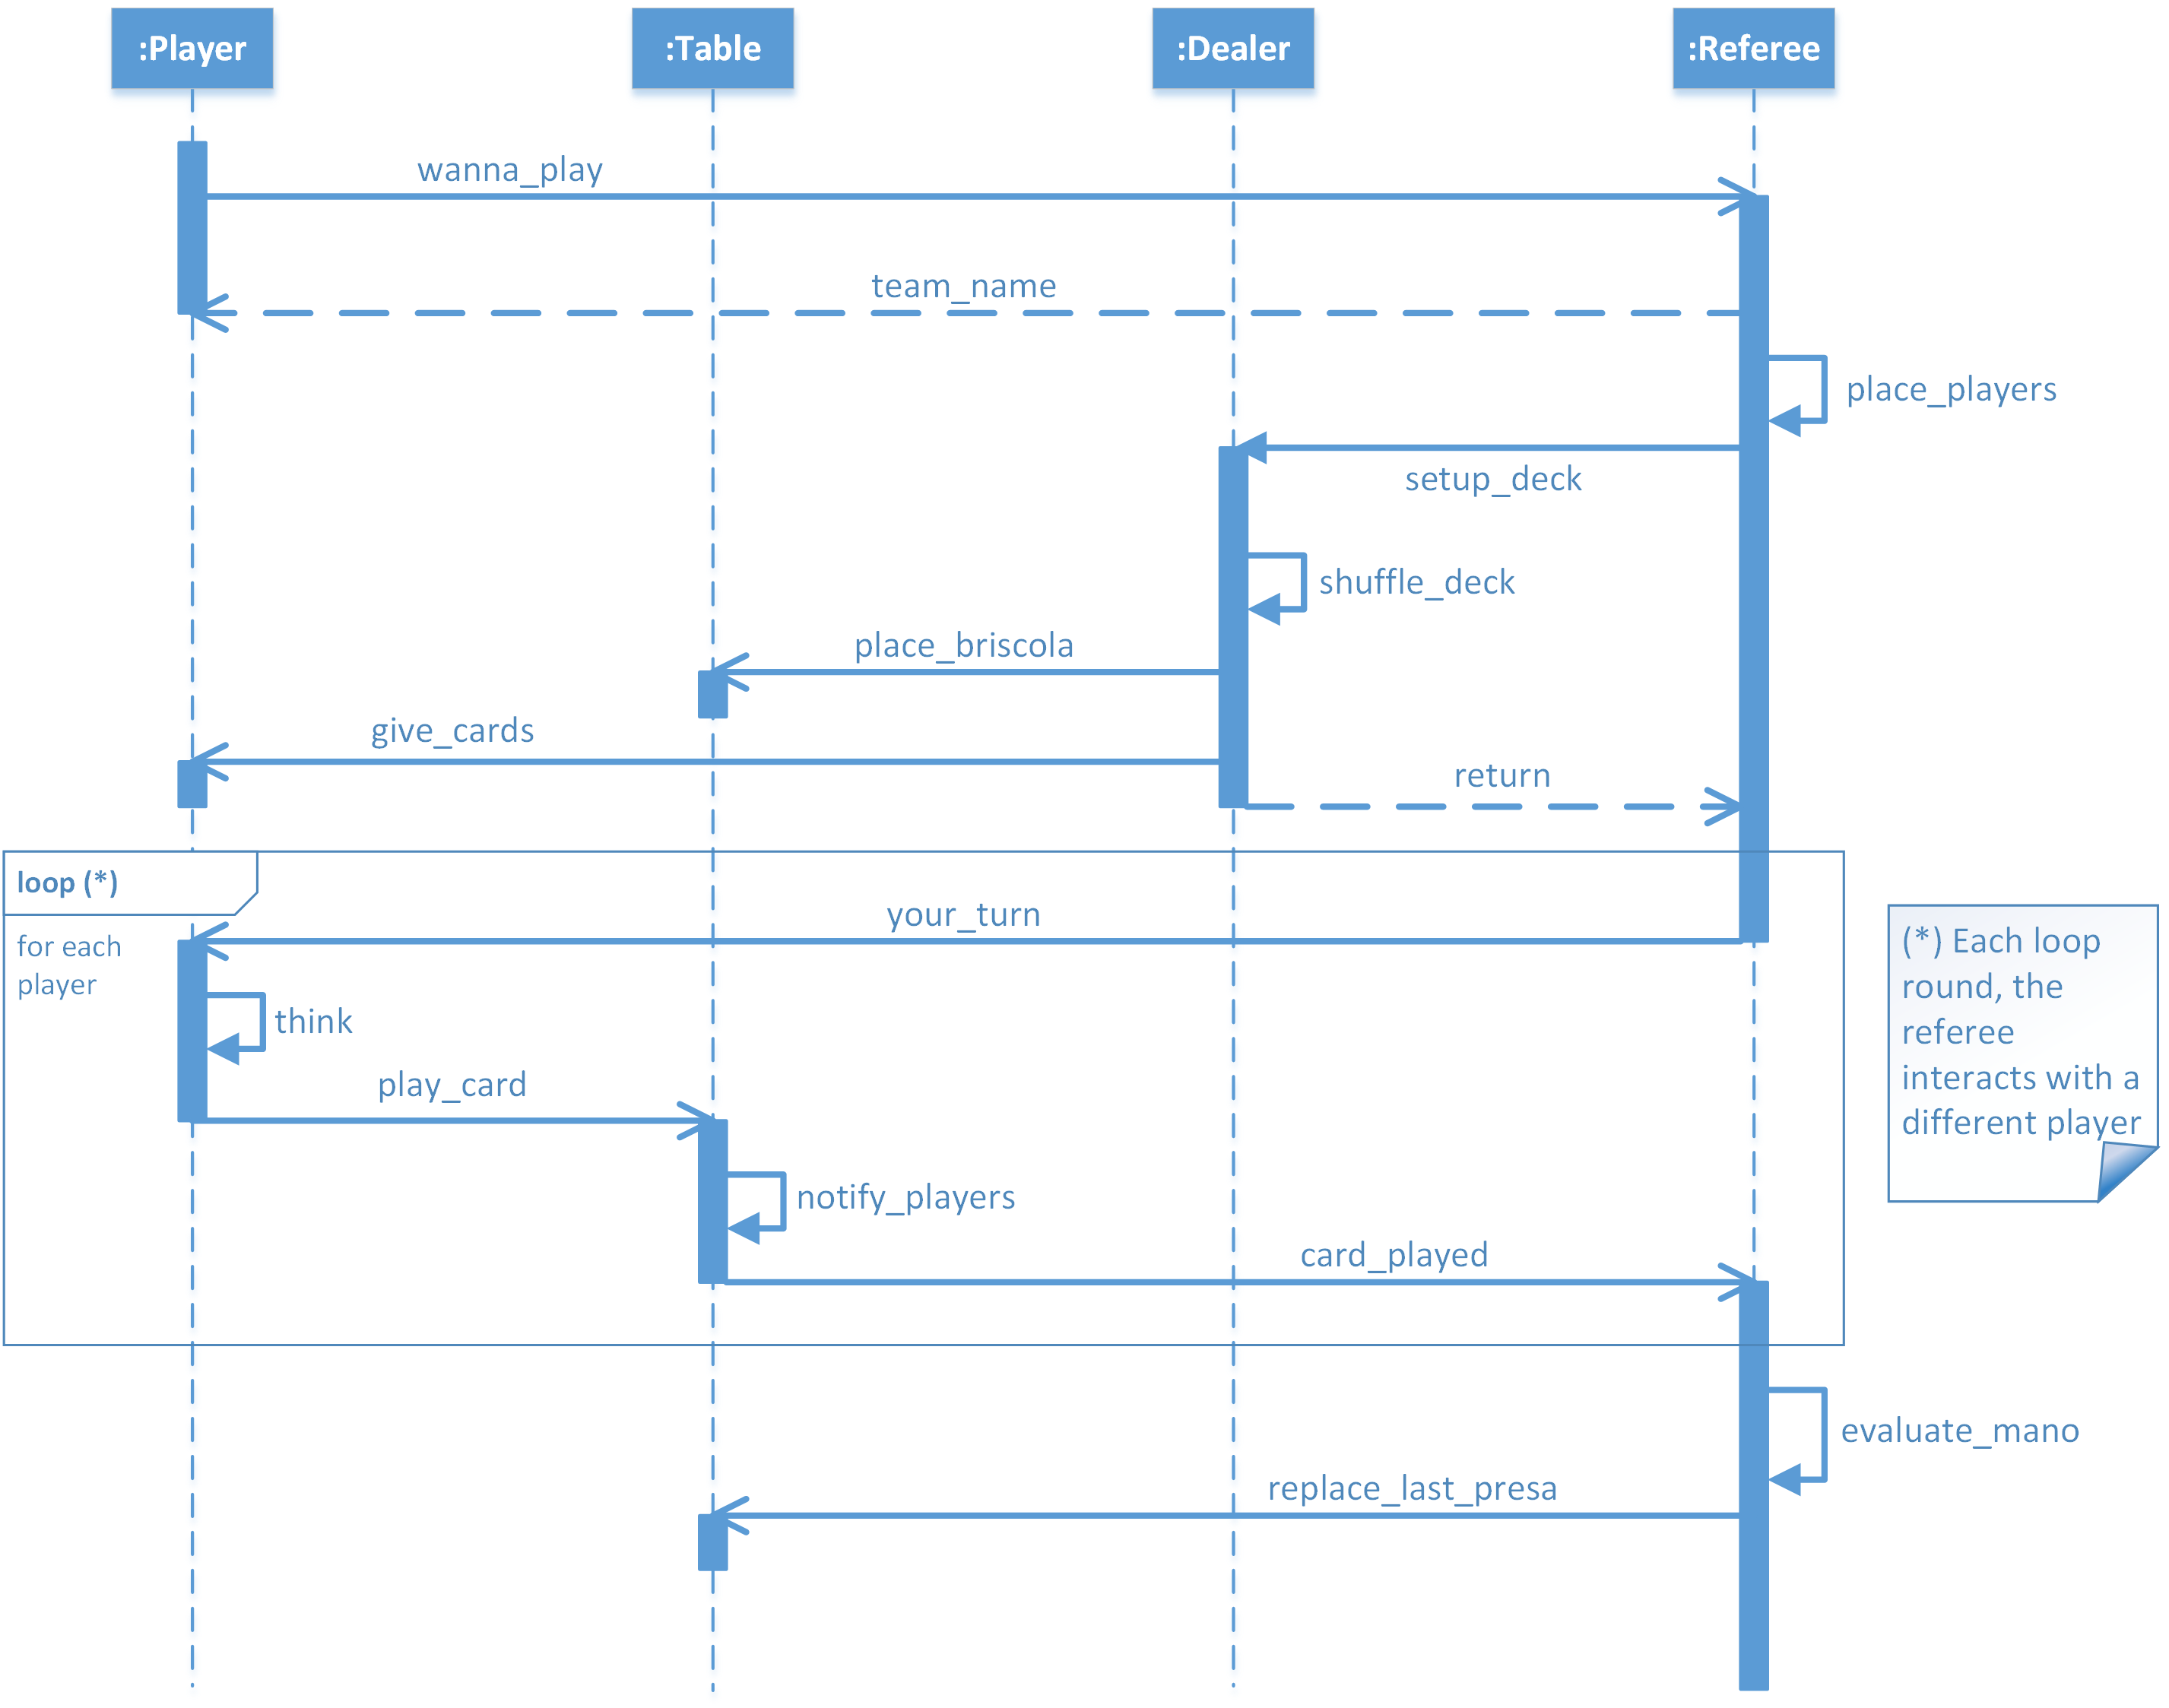
\includegraphics[width=180mm]{./img/general_sequence_diagram.png}
	\caption{Diagramma di sequenza del sistema per il primo turno. Per motivi grafici non sono stati inclusi nella rappresentazione tutti i giocatori di una partita, ma solamente uno di essi. \label{general-sequence-diagram}}
\end{figure}

Le mani successive sono molto simili alla prima, anche se presentano una meccanica aggiuntiva: i primi giocatori di ogni squadra hanno la possibilità di parlare con il compagno. La dinamica che descrive lo svolgimento di tale azione non è stata approfondita in maniera adeguata nella fase di analisi dei requisiti in \autoref{requirements-analysis}. Essa può essere modellata attraverso due principali schemi di interazione:
\begin{itemize}
	\item \textbf{Comunicazione diretta}: la soluzione più semplice consiste nel fare in modo che il giocatore che parla comunichi in modo diretto la propria domanda sia al compagno di squadra, sia ai giocatori avversari. La risposta, allo stesso modo, deve essere trasmessa a tutti i giocatori.
	\item \textbf{Comunicazione mediata}: in questo caso si considera l'etere come lo spazio nel quale avviene la comunicazione. Un giocatore quando parla trasmette le proprie informazioni nell'ambiente in cui si svolge la partita. La domanda posta dal giocatore è rivolta al compagno di gioco, ma può essere recepita da tutte le entità situate nell'ambiente circostante. Solo il compagno sarà responsabile di rispondere alla domanda, propagando l'informazione sullo spazio comune tra i giocatori.
\end{itemize}
La seconda opzione implica una rivisitazione del modello del sistema abbozzato fino ad ora, ma garantisce un grado di disaccoppiamento tra i giocatori. In questo caso, una nozione di \emph{situatedness} si rivela determinante per il sistema. Ogni giocatore risulta situato in un ambiente di gioco, nel quale può consultare le carte che si trovano sul tavolo ed è in grado di recepire tutte le informazioni emesse dagli altri giocatori. In questo contesto, l'ambiente di gioco deve necessariamente essere considerato come un'astrazione di primo ordine, attraverso l'introduzione nel sistema di un nuovo componente, il \emph{game environment}. Esso include al suo interno anche il tavolo da gioco, che non è altro che una astrazione attraverso la quale ogni giocatore interagisce con l'ambiente, ricevendo da essa delle informazioni che influiscono sul proprio comportamento e agendo in modo da cambiare lo stato del mondo corrente. 

Ogni giocatore interagisce costantemente con il \emph{game environment}, sia per quanto riguarda le azioni relative al tavolo da gioco (come consultazione della mano corrente, giocata di una carta, \dots), sia per quanto riguarda la trasmissione delle informazioni quando un giocatore parla. L'interazione tra il tavolo e gli altri componenti del sistema è stata già affrontata e sviscerata in precedenza e non necessita di essere riveduta. Risulta diverso, invece, il discorso relativo all'azione di parlare, la cui dinamica è rappresentata nel diagramma di sequenza in \autoref{}.


\section{Studio di fattibilità}
\subsection{Componenti}
Tutti i componenti, ad esclusione del tavolo da gioco, sono stati identificati come entità attive. Le soluzioni più consone per la modellazione di tali componenti ricadono nell'utilizzo degli attori o degli agenti. Infatti, queste astrazioni si basano sul fatto che ogni componente sia contraddistinto da un proprio flusso di controllo (logico o fisico) e risultano quindi ideali per l'implementazione di giocatori, mazziere e arbitro.

Il tavolo da gioco è un componente passivo con il quale è possibile interagire tramite chiamate ai metodi che esso metterà a disposizione.

\subsection{Interazione}
% Studiare la fattiilità delle comunicazioni/interazioni, concludendo che l'utilizzo di uno spazio di tuple è la soluzione migliore.
Come espresso in precedenza, i requisiti non pongono vincoli sulle modalità di interazione dei componenti. Segue uno studio sulle possibili strategie adottabili per far fronte a tale questione.

\begin{description}
	\item[Scambio di messaggi]:
\end{description}

\section{Design architetturale} \label{design}

\fancyhead{}
\renewcommand{\headrulewidth}{0pt}
\appendix
\addcontentsline{toc}{section}{Appendice}
\section*{Appendice}

\subsection*{Regole del gioco della briscola - 4 giocatori}\label{briscola-rules}

Non avendo trovato un regolamento ufficiale, si è preso come riferimento quello generale riportato in \footnote{\url{https://it.wikipedia.org/wiki/Briscola}}, con qualche piccola variazione.
 
I giocatori giocano in coppie di due, con un mazzo di 40 carte regionali. I punti disponibili per ogni partita sono in totale 120, vince chi ne realizza almeno 61; se i punti sono 60 per entrambe le coppie, la partita è pareggiata. I valori di presa sono nell'ordine decrescente: Asso, 3, Re, Cavallo, Donna o Fante, 7, 6, 5, 4 e 2. I giocatori devono essere disposti facendo sì che ognuno di essi abbia ai suoi lati i giocatori della squadra avversaria, in modo che due giocatori della stessa squadra non giochino mai consecutivamente. Disposti i giocatori, il mazziere mischia le carte senza guardare il mazzo, distribuisce 3 carte ciascuno e lascia una carta sul tavolo coprendola per metà con il mazzo posto trasversalmente ad essa, in modo che rimanga visibile a tutti per l'intero gioco: questa carta segnerà il seme di briscola e sarà l'ultima carta ad essere pescata. Partendo dal primo giocatore (quello che ha ricevuto la prima carta) e continuando in senso antiorario. Ogni giocatore calerà la carta che riterrà più opportuna, con lo scopo di aggiudicarsi la mano o di totalizzare il maggior numero di punti assieme al proprio compagno. Da parte dei giocatori non esiste alcun obbligo di giocare un particolare tipo di seme. L'aggiudicazione della mano avviene secondo regole molto semplici:
\begin{itemize}
	\item il primo giocatore di mano determina il seme di mano calando la sua carta, detta dominante, e virtualmente è il vincitore temporaneo della mano.
	\item la mano può essere temporaneamente aggiudicata ad un altro giocatore se questi posa una carta del seme di mano con valore di presa maggiore (si dice che il giocatore ha "strozzato" la dominante), oppure giocando una qualsiasi carta del seme di briscola, anche con valore di presa inferiore rispetto alla carta dominante. Bisogna sottolineare che non vi è obbligo di risposta al seme della dominante.
\end{itemize}
Alla fine la mano è vinta dal giocatore che ha calato la carta di briscola col valore di presa maggiore o, in mancanza di questa, dal giocatore che ha calato la carta del seme di mano con il valore di presa maggiore. Se nessuno ha strozzato la dominante e se nessuno ha giocato una briscola, la mano è vinta dal primo giocatore di mano. Il giocatore che vince la mano prende tutte le carte poste sul tavolo e le ripone coperte davanti a sé; in seguito sarà il primo a prendere la prima carta dal mazziere, seguito da tutti gli altri sempre in senso antiorario e sarà il primo ad aprire la mano successiva e quindi a decidere il nuovo seme di mano. Alla prima mano è vietato parlare, diversamente dal resto della partita dove si può parlare. Quando il mazziere esaurisce le carte, i giocatori continuano a giocare fino ad esaurire le carte che hanno in mano. A quel punto la partita termina e si procede al conteggio dei punti (in una partita a 4 giocatori, una partita termina dopo 10 mani di gioco). Il punteggio di una squadra è dato dalla somma dei punti dei due giocatori che ne fanno parte. I punteggi delle carte sono riportate di seguito:

\begin{center}
	\begin{tabular}{| l | l | l | l | l | l | l |}
		\hline
		\textbf{Carte} & Asso & 3 & Re & Cavallo & Fante & 7-2 \\ \hline
		\textbf{Punti} & 11 & 10 & 4 & 3 & 2 & 0 \\ 
		\hline
	\end{tabular}
\end{center}

Durante lo svolgimento della partita, alle squadre non è consentito consultare le proprie prese dei turni precedenti per conteggiare i punti guadagnati. Tuttavia, in ogni momento, entrambe le squadre hanno diritto a consultare l'ultima presa che è stata fatta, ovvero quella della mano precedente.

\end{document}
